%
% chapter.tex -- Beschreibung des Inhaltes
%
% (c) 2021 Prof Dr Andreas Müller, Hochschule Rapperswil
%
% !TeX spellcheck = de_CH
\chapter{Spezielle Funktionen aus der Geometrie
\label{buch:chapter:geometrie}}
\lhead{Spezielle Funktionen aus der Geometrie}
\rhead{}

Die ältesten geometrisch definierten speziellen Funktionen
sind die Wurzeln.
Sie haben ermöglicht, die Kantenlänge eines Quadrates mit vorgegebenem
Flächeninhalt zu bestimmen.
Die Formel von Pythagoras über die Seitenlängen eines rechtwinkligen
Dreiecks ermöglicht, mit Hilfe von Quadratwurzeln aus zwei Seiten
die dritte zu berechnen.
Der Strahlensatz schliesslich reduziert alle rechtwinkligen
Dreiecke auf spezielle Dreiecke, deren eine Seite Einheitslänge 
hat.
Die Seitenverhältnisse in einem rechtwinkligen Dreieck hängen nur 
vom Winkel ab.
Dies führt auf eine neue Klasse von speziellen Funktionen,
die trigonometrischen Funktionen,
die ebenfalls bereits im Altertum bekannt waren.

Mindestens ebenso wichtig wie die Berechnung ebener Dreieck
war im Altertum aber die Berechnung von Dreiecken am Himmel.
Auf einer Kugeloberfläche funktioniert Ähnlichkeit nicht mehr,
der Strahlensatz muss durch den Satz von Menelaos ersetzt werden.
Es ergibt sich eine Methode, beliebige Dreiecke auf einer Kugeloberfläche
ganz analog zum Vorgehen bei ebenen Dreiecken zu berechnen.
Diese sphärische Trigonometrie ist die Basis der Navigation
und aller astrometrischer Berechnungen.

Die Analysis hat die Möglichkeit geschaffen, die Länge von Kurven
zu definieren und zu berechnen, wie auch den Flächeninhalt von
Gebieten, die von Kurven berandet sind.
Es stellt sich heraus, dass bereits anscheinend einfache Aufgaben
wie die Berechnung der Länge von Ellipsen- oder Hyperbelbögen auf
die Notwendigkeit führt, neue spezielle Funktionen zu definieren.

%
% trigonometrisch.tex
%
% (c) 2021 Prof Dr Andreas Müller, OST Ostschweizer Fachhochschule
%
\section{Trigonometrische Funktionen
\label{buch:geometrie:section:trigonometrisch}}
\rhead{Trigonometrische Funktionen}
Die Navigation zur See wie auch die Landvermessung hängen davon ab,
dass man Winkel zwischen Himmelskörpern, Landmarken oder dem Horizont
messen kann.
Aus solchen Messungen können dann mittels bekannter Beziehungen
zwischen den Winkeln und Seitenlängen in Dreiecken weitere Seitenlängen
und Winkel berechnet werden.
Schon in rechtwinkligen Dreiecken sind die Beziehungen zwischen Winkel
und Seitenlängen von einer Art, die sich nicht durch algebraische
Ausdrücke berechnen lässt.
Es ist daher notwendig, neue spezielle Funktionen zu definieren,
die trigonometrischen Funktionen.

\subsection{Definition der trigonometrischen Funktionen}
% XXX Abbildung Jakobsstab
Eines der ältesten Messgeräte für Winkel ist der Jakobsstab,
dargestellt in Abbildung~\ref{}.
Der Querstab kann entlang des Stabs verschoben werden.
Die beiden Punkte, deren Zwischenwinkel bestimmt werden soll,
werden so anvisiert, dass sie sich auf den Enden des Querstabs 
zu befinden scheinen.
Abgelesen wird dann die Strecke $l$ zwischen dem Auge des Beobachters
und dem Querstab.
Daraus und aus der Länge $l_Q$ des Querstabes lässt sich jetzt der Winkel
mit der Formel
\[
\tan\frac{\alpha}2 = \frac{l_Q}{2l}
\]
berechnen.
Um nun einen numerischen Wert für $\alpha$ zu bekommen, braucht man
eine Tabelle der Funktionswerte der Funktion auf der linken Seite.

\begin{figure}
\centering
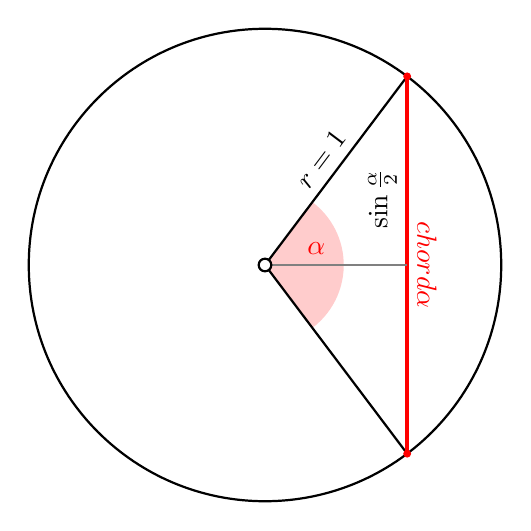
\begin{tikzpicture}[>=latex,thick]
\def\r{3}
\def\a{53}
\fill[color=red!20] (0,0) -- (-\a:1) arc (-\a:\a:1) -- cycle;
\draw (0,0) -- (\a:\r);
\draw (0,0) -- (-\a:\r);
\node[color=red] at ({cos(\a/2)},0) [above left] {$\alpha$};
\draw (0,0) circle[radius=\r];
\draw[color=red,line width=1.4pt] (\a:\r) -- (-\a:\r);
\fill[color=red] (\a:\r) circle[radius=0.05];
\fill[color=red] (-\a:\r) circle[radius=0.05];
\node[color=red] at ({\r*cos(\a)},0)
	[above,rotate=-90] {$\operatorname{chord}\alpha$};
\draw[color=gray,line width=1.0pt] (0,0) -- ({\r*cos(\a)},0);
\fill[color=white] (0,0) circle[radius=0.08];
\draw (0,0) circle[radius=0.08];
\node at (\a:{0.5*\r}) [above,rotate=\a] {$r=1$};
\node at ({\r*cos(\a)},{0.35*\r*sin(\a)})
	[above,rotate=90] {$\sin\frac{\alpha}2$};
\end{tikzpicture}
\caption{Definition der Chord-Funktion $\operatorname{chord}\alpha$
am Einheitskreis.
\label{buch:geometrie:trigo:chorddef}}
\end{figure}

Die älteste bekannt Tabelle von Funktionswerten trigonometrischer
Funktionen stammt von Hipparchus aus dem 2.~Jahrhundert BCE und
enthält Werte der sogenannten Chord-Funktion $\operatorname{chord}\alpha$,
welche die Länge der Sehne eines Bogens $\alpha$ des Einheitskreises
berechnet.
Aus der Abbildung~\ref{buch:geometrie:trigo:chorddef} ergibt sich
\[
\operatorname{chord}\alpha = 2\sin\frac{\alpha}2.
\]
Die Verwendung der Chord-Funktion war bis ins 19.~Jahrhundert in der
Landvermessung üblich.
Neben der Chord-Funktion waren auch noch andere heute weitgehend
vergessen Funktionen im Einsatz wie zum Beispiel der Sinus versus
\[
\operatorname{vers}\alpha=1-\cos\alpha
=
2\sin^2\frac{\alpha}2
\]
oder der Semiversus
\[
\operatorname{sem}\alpha
=
\frac{\operatorname{vers}\alpha}{2}
=
\sin^2\frac{\alpha}2,
\]
der besonders nützlich bei der Berechnung der Entfernung
zweier in geographischer Länge und Breite gegebener Punkte
auf der Erdoberfläche ist und daher in der Navigation lange
üblich war.

Eine neue spezielle Funktion sollte sowohl möglichst
universell einsetzbar sein als auch gut und effizient
berechnet werden können.
Aus dieser Forderung haben sich die Funktion $\sin\alpha$,
$\cos\alpha$ und $\tan\alpha$ als die nützlichsten herausgestellt.
Mit ihnen lassen sich a

%
% Rechtwinklige Dreiecke
%
\subsubsection{Rechtwinklige Dreiecke}
Ähnliche Dreiecke haben gleiche Seitenverhältnisse und Winkel.
Rechtwinklige Dreiecke sind daher bis auf Ähnlichkeit vollständig
durch die Angabe eines Winkels beschrieben.
Die Seitenverhältnisse müssen daher aus den Winkeln berechnet werden
können.
Genau dies ist die Aufgabe, die die trigonometrischen Funktionen lösen.

\begin{figure}
\centering
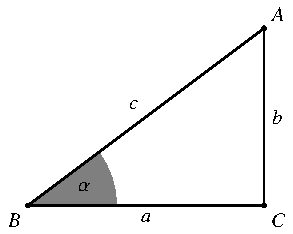
\includegraphics{chapters/030-geometrie/images/deftrig.pdf}
\caption{Rechtwinkliges Dreieck zur Definition der trigonometrischen
Funktionen.
\label{buch:geometrie:trigo:fig:definition}}
\end{figure}

\begin{definition}
\label{buch:geometrie:def:trigo}
In einem rechtwinkligen Dreieck mit Winkel $\alpha$, $0<\alpha < \frac{\pi}2$,
sind die Seitenverhältnisse gegeben durch die trigonometrischen Funktionen,
die wie folgt definiert sind:
\begin{align*}
\sin\alpha &= \frac{\text{Gegenkatete}}{\text{Hypothenuse}} = \frac{b}{c},
&
\cos\alpha &= \frac{\text{Ankatete}}{\text{Hypothenuse}} = \frac{a}{c}
&&\text{und}
&
\tan\alpha &= \frac{\text{Gegenkatete}}{\text{Ankatete}} = \frac{a}{b}
\intertext{mit den Kehrwerten}
\sec\alpha &= \frac{\text{Hypothenuse}}{\text{Gegenkatete}} = \frac{c}{b},
&
\csc\alpha &= \frac{\text{Hypothenuse}}{\text{Ankatete}} = \frac{c}{a}
&&\text{und}
&
\cot\alpha &= \frac{\text{Ankatete}}{\text{Gegenkatete}} = \frac{b}{a}
\end{align*}
(siehe auch Abbildung~\ref{buch:geometrie:trigo:fig:definition}).
\end{definition}

Aus der Definition und dem Satz von Pythagoras kann eine grosse Zahl
von Beziehungen zwischen den trigonometrischen Funktionen abgeleitet
werden.
Zum Beispiel folgt sofort
\[
\sin^2\alpha+\cos^2\alpha
=
\biggl(\frac{b}{c}\biggr)^2
+
\biggl(\frac{a}{c}\biggr)^2
=
\frac{a^2+b^2}{c^2} 
=
1.
\]
Insbesondere lässt sich $\sin\alpha$ durch $\cos\alpha$ ausdrücken
und umgekehrt:
\[
\sin\alpha
=
\sqrt{1-\cos^2\alpha}
\qquad\text{und}\qquad
\cos\alpha
=
\sqrt{1-\sin^2\alpha}
\]
Da sich alle Funktionen durch $\cos\alpha$ und $\sin\alpha$ ausdrücken
lassen, können alle auch nur durch eine ausgedrückt werden.
Durch Umkehrung dieser Beziehung kann man jede der trigonometrischen
Funktionen durch jede andere ausdrücken, wie dies in
Tabelle~\ref{buch:geometrie:tab:trigo} zusammengestellt ist.

\begin{figure}
\centering
\renewcommand{\arraystretch}{2.5}
\renewcommand{\tabcolsep}{5pt}
\begin{tabular}{|>{$}c<{$}|>{$}c<{$}>{$}c<{$}>{$}c<{$}>{$}c<{$}>{$}c<{$}>{$}c<{$}|}
\hline
%\downarrow\text{ ausgedrückt durch }\rightarrow
&\sin\alpha&\cos\alpha&\tan\alpha&\cot\alpha&\sec\alpha&\csc\alpha\\[5pt]
\hline
\sin\alpha
	&\sin\alpha
	&\sqrt{1-\cos^2}
		&\displaystyle\frac{\tan\alpha}{\sqrt{1+\tan^2\alpha}}
		&\displaystyle\frac{1}{\sqrt{1+\cot^2\alpha}}
			&\displaystyle\frac{1}{\sec\alpha}
			&\displaystyle\frac{\sqrt{\csc^2\alpha-1}}{\csc\alpha}
\\
\cos\alpha
	&\sqrt{1-\sin^2\alpha}
	&\cos\alpha
		&\displaystyle\frac{1}{\sqrt{1+\tan^2\alpha}}
		&\displaystyle\frac{\cot\alpha}{\sqrt{1+\cot^2\alpha}}
			&\displaystyle\frac{\sqrt{\sec^2\alpha-1}}{\sec\alpha}
			&\displaystyle\frac{1}{\csc\alpha}
\\
\tan\alpha
	&\displaystyle\frac{\sin\alpha}{\sqrt{1-\sin^2\alpha}}
	&\displaystyle\frac{\sqrt{1-\cos^2\alpha}}{\cos\alpha}
		&\tan\alpha
		&\displaystyle\frac{1}{\cot\alpha}
			&\displaystyle\frac{1}{\sqrt{\sec^2\alpha-1}}
			&\displaystyle\sqrt{\csc^2\alpha-1}
\\
\cot\alpha
	&\displaystyle\frac{\sqrt{1-\sin^2\alpha}}{\sin\alpha}
	&\displaystyle\frac{\cos\alpha}{\sqrt{1-\cos^2\alpha}}
		&\displaystyle\frac{1}{\tan\alpha}
		&\cot\alpha
			&\displaystyle\sqrt{\sec^2\alpha-1}
			&\displaystyle\frac{1}{\sqrt{\sec^2\alpha-1}}
\\
\sec\alpha
	&\displaystyle\frac{1}{\sin\alpha}
	&\displaystyle\frac{1}{\sqrt{1-\cos^2\alpha}}
		&\displaystyle\frac{\sqrt{1+\tan^2\alpha}}{\tan\alpha}
		&\displaystyle\sqrt{1+\cot^2\alpha}
			&\sec\alpha
			&\displaystyle\frac{\csc\alpha}{\sqrt{\csc^2\alpha-1}}
\\
\csc\alpha
	&\displaystyle\frac{1}{\sqrt{1-\sin^2\alpha}}
	&\displaystyle\frac{1}{\cos\alpha}
		&\displaystyle\sqrt{1+\tan^2\alpha}
		&\displaystyle\frac{\sqrt{1+\cot^2\alpha}}{\cot\alpha}
			&\displaystyle\frac{\sec\alpha}{\sqrt{\sec^2\alpha-1}}
			&\csc\alpha
\\[8pt]
\hline
\end{tabular}
\caption{Darstellung aller trigonometrischen Funktionen durch jede beliebige
andere Funktion.
Für Winkel ausserhalb des 1.~Quadranten müssen die Vorzeichen der
Quadratwurzeln so gewählt werden, dass die Funktion das richtige
Vorzeichen erhält.
\label{buch:geometrie:tab:trigo}}
\end{figure}

Diese Definition~\ref{buch:geometrie:def:trigo}
ist auf spitze Winkel und damit auf nichtnegative Werte der
trigonometrischen Funktionen beschränkt.

%
% Definition am Einheitskreis
%
\subsubsection{Einheitskreis}
Im vorangegangen Abschnitt wurden die rechtwinkligen Dreiecke durch
einen Winkel charakterisiert und die trigonometrischen
Funktionen als Verhältnis von Seiten des Dreiecks abgeleitet.
Dabei wurde die Schwierigkeit übergangen, wie überhaupt der Winkel
definiert werden soll.
Ein Winkel war im Wesentlichen durch die Eigenschaft
definiert, dass ähnliche Dreiecke den gleichen Winkel haben.
Die Definition~\ref{buch:geometrie:def:trigo} ist in diesem Licht
nichts anderes als eine Namenskonvention für die Seitenverhältnisse
einer Klasse von ähnlichen rechtwinkligen Dreiecken.

\begin{figure}
\centering
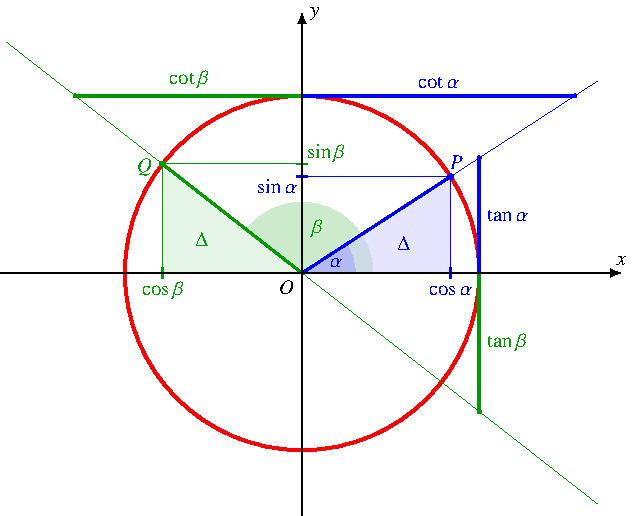
\includegraphics{chapters/030-geometrie/images/einheitskreis.pdf}
\caption{Definition der trigonometrischen Funktion mit Hilfe des
Einheitskreises
\label{buch:geometrie:trigo:fig:einheitskreis}}
\end{figure}

Eine alternative Charakterisierung rechtwinkliger Dreiecke
geht von Punkten auf dem Einheitskreis aus.
Die Lote von einem Punkt $P$ auf dem Einheitskreis definieren
zwei ähnliche Dreiecke, mit dem Ursprung $O$, dem Punkt $P$
und dem Fusspunkt des Lotes.
Die Koordinaten des Punktes $P$ können im Gegensatz zu den Seiten
des rechtwinkligen Dreiecks in
Abbildung~\ref{buch:geometrie:trigo:fig:definition}
auch negativ sein.
Ein Punkt im zweiten Quadranten hat zum Beispiel eine negative
$x$-Koordinate.
Die trigonometrischen Funktionen können nun analog zu
Definition~\ref{buch:geometrie:def:trigo} aber unter Verwendung
der Koordinaten $x$ und $y$.

Auch das Argument $\alpha$ der trigonometrischen Funktionen kann
jetzt auf natürlichere Art und Weise definiert werden.
Es ist die Länge des Bogens auf dem Einheitskreis zwischen dem
Punkt $(1,0)$ und $P$.
Damit lassen sich die trigonometrischen Funktionen jetzt
für beliebige Winkel $\alpha\in\mathbb{R}$ definieren.

\begin{definition}
\label{buch:geometrie:def:trigeinheitskreis}
Die trigonometrischen Funktionen des Winkels $\alpha$ zwischen der 
$x$-Achse und der Richtung durch den Punkt $P$ sind 
\begin{align*}
\sin\alpha &= x, &\cos\alpha &= y&&\text{und}& \tan\alpha=\frac{y}{x}
\intertext{mit den Kehrwerten}
\sec\alpha &= \frac{1}{x}, &\csc\alpha &= \frac{1}{y}&&\text{und}& \tan\alpha=\frac{x}{y}.
\end{align*}
(siehe auch Abbildung~\ref{buch:geometrie:trigo:fig:einheitskreis}).
\end{definition}

Die Beziehungen der Tabelle~\ref{buch:geometrie:tab:trigo}
zwischen den trigonometrischen Funktionen bleibt auch für 
diese erweiterten Funktionen gültig, wenn das Vorzeichen der
Quadratwurzel falls vorhanden geeignet gewählt wird.

%
% Drehungen in der Ebene
%
\subsection{Drehungen der Ebene}
Die Funktionen $\sin\alpha$ und $\cos\alpha$ sind in den Anwendungen
besonders nützlich, weil sich damit die Kreisbewegung parametrisieren
lässt.
Etwas allgemeiner kann man damit Drehungen der Ebene beschreiben.
Damit entstehen die Funktion als Nebenprodukt einer Parametrisierung
der Drehgruppe $\operatorname{SO}(2)$.
Daraus werden sich später Ableitungseigenschaften und
Potenzreihendarstellungen der trigonometrischen Funktionen ableiten
lassen.

\subsubsection{Drehmatrizen und Additionstheoreme}
Eine Drehung der Ebenen $\mathbb{R}^2$ um den Winkel $\alpha$ bildet
die Standardbasisvektoren auf die Vektoren
\[
e_1=\begin{pmatrix}1\\0\end{pmatrix}
\mapsto
\begin{pmatrix}
\cos\alpha\\\sin\alpha
\end{pmatrix}
\qquad\text{und}\qquad
e_2=\begin{pmatrix}0\\1\end{pmatrix}
\mapsto
\begin{pmatrix}
-\sin\alpha
\\
\cos\alpha
\end{pmatrix}
\]
ab.
Die Abildungsmatrix der Drehung ist daher
\[
D_\alpha
=
\begin{pmatrix*}[r]
\cos\alpha&-\sin\alpha\\
\sin\alpha& \cos\alpha
\end{pmatrix*}.
\]
Die Zusammensetzung zweier Drehungen um die Winkel $\alpha$ und $\beta$
ist wieder eine Drehung um den Winkel $\alpha+\beta$, es gilt
also
\[
D_{\alpha+\beta}
=
D_{\alpha}D_{\beta},
\]
oder in Matrizenform
\begin{align*}
D_{\alpha+\beta}
&=
\begin{pmatrix*}[r]
\cos(\alpha+\beta)&-\sin(\alpha+\beta) \\
\sin(\alpha+\beta)& \cos(\alpha+\beta)
\end{pmatrix*}
\\
=
D_{\alpha}D_{\beta}
&=
\begin{pmatrix*}[r]
\cos\alpha&-\sin\alpha\\
\sin\alpha&\cos\alpha
\end{pmatrix*}
\begin{pmatrix*}[r]
\cos\beta&-\sin\beta\\
\sin\beta&\cos\beta
\end{pmatrix*}
\\
&=
\begin{pmatrix}
\cos\alpha\cos\beta-\sin\alpha\sin\beta
	& -\cos\alpha\sin\beta -\sin\alpha\cos\beta\\\
\cos\alpha\sin\beta+\sin\alpha\cos\beta
	& \cos\alpha\cos\beta-\sin\alpha\sin\beta
\end{pmatrix}
\end{align*}
Aus dem Vergleich der beiden Matrizen liest man die Additionstheoreme.

\begin{satz}
Für $\alpha,\beta\in\mathbb{R}$ gilt
\begin{align*}
\sin(\alpha\pm\beta)
&=
\cos\alpha\cos\beta\mp\sin\alpha\sin\beta
\\
\cos(\alpha\pm\beta)
&=
\cos\alpha\cos\beta\pm\sin\alpha\sin\beta
\end{align*}
\end{satz}

Ein besonders einfacher Spezialfalls ist $\alpha=\beta$, es ergben sich die
Doppelwinkelformeln
\begin{align*}
\cos2\alpha &= \cos^2\alpha-\sin^2\alpha
\\
\sin2\alpha &= 2\cos\alpha\sin\alpha.
\end{align*}
In der Formel für $\cos2\alpha$ kann die rechte Seite durch nur
eine Winkelfunktion ausdrücken:
\begin{align*}
\cos2\alpha &= \cos^2\alpha - (1-\cos^2\alpha) = 2\cos^2\alpha -1
\\
\cos2\alpha &= (1-\sin^2\alpha) - \sin^2\alpha = 1-2\sin^2\alpha.
\end{align*}
Beide Ausdrücke lassen sich leicht nach den Funktionen auf der rechten
Seite auflösen, so erhält man die Halbwinkelformeln
\begin{align*}
\cos^2\alpha &= \frac{1+\cos2\alpha}2
&&\Rightarrow&
\cos^2\frac{\alpha}2 &=\frac{1+\cos\alpha}2
\\
\sin^2\alpha &= \frac{1-\sin2\alpha}2
&&\Rightarrow&
\sin^2\frac{\alpha}2 &= \frac{1-\sin\alpha}2.
\end{align*}
Der letzte Ausdruck ist auch bekannt als der Semiversus.

\subsubsection{Funktionen für mehrfache Winkel}
Die Additionstheoreme können dazu verwendet werden, Formeln für
die Werte der trigonometrischen Funktionen mehrfacher Winkel zu
finden.
Die Berechnung kann etwas vereinfacht werden, wenn man die Drehmatrix
mit Hilfe der Matrix
\[
J=\begin{pmatrix}0&-1\\1&0\end{pmatrix}
\]
als
\[
D_{\alpha}
=
E
\cos\alpha
+
J
\sin\alpha
\]
schreiben.
Die Potenzen von $J$ sind
\[
J^2 = -E,\quad
J^3 = -J \quad\text{und}\quad
J^4 = E.
\]
Daraus ergibt sich
\begin{align*}
D_{n\alpha}
=
(D_{\alpha})^n
&=
(E\cos\alpha+J\sin\alpha)^n
\\
&=
\sum_{k=0}^n \binom{n}{k}\cos^{n-k}\alpha\sin^{k}\alpha J^k
\\
&=
\sum_{l=0}^{\lfloor\frac{n}2\rfloor}
(-1)^l
\binom{n}{2l}\cos^{n-2l}\alpha \sin^{2l}\alpha 
-
J
\sum_{l=0}^{\lfloor\frac{n}2\rfloor}
(-1)^l
\binom{n}{2l+1}\cos^{n-2l-1}\alpha \sin^{2l+1}\alpha 
\intertext{Durch Vergleich mit der Matrix $D_{n\alpha}$ findet man die
Formeln für die Funktionen des $n$-fachen Winkels:}
\cos n\alpha
&=
\sum_{l=0}^{\lfloor\frac{n}2\rfloor}
(-1)^l
\binom{n}{2l}\cos^{n-2l}\alpha \sin^{2l}\alpha 
\\
\sin n\alpha
&=
-
\sum_{l=0}^{\lfloor\frac{n}2\rfloor}
(-1)^l
\binom{n}{2l+1}\cos^{n-2l-1}\alpha \sin^{2l+1}\alpha 
\end{align*}
Für kleine Werte von $n$ sind die Formeln einigermassen übersichtlich,
zum Beispiel für $n=3$:
\begin{align*}
\cos 3\alpha
&=
\cos^3\alpha-3\cos\alpha\sin^2\alpha
=
\cos^3\alpha-3\cos\alpha(1-\cos^2\alpha)
\\
&=
4\cos^3\alpha-3\cos\alpha,
\\
\sin 3\alpha
&=
3\cos^2\alpha\sin\alpha
-
\sin^3\alpha
=
3(1-\sin^2\alpha)\sin\alpha-\sin^3\alpha
\\
&=
-4\sin^3\alpha
+3\sin\alpha.
\end{align*}
Indem man diese Formeln als kubische Gleichungen für die
Unbekannte $\cos\alpha$ bzw.~$\sin\alpha$ betrachtet, kann
man durch Lösung der Gleichung zum Beispiel mit der Formel von
Cardano 
% XXX Verweis auf die Formel von Cardano
zu gegebenen Werten von $\cos 3\alpha$ und $\sin 3 \alpha$
die Werte von $\cos\alpha$ und $\sin\alpha$ durch rein
algebraische Operationen bestimmen.

\subsubsection{Eine Tabelle der Werte der trigonometrischen Funktionen
aufstellen}
Die älteste Tabelle der Werte trigonometrischer Funktionen stammt aus der
Feder von Hipparcos aus dem zweiten Jahrhundert BCE.
Sie hatte eine Auflösung von $1^\circ$.
Wie kann man eine solche Tabelle mit den Mitteln der damaligen Zeit,
also insbesondere ganz ohne Dezimalbrüche, zusammenstellen?

Aus speziellen Dreiecken kann man die einige wenige bekannte Winkel
finden und die zugehörigen Werte der trigonemetrischen Funktionen
bestimmen.
In einem rechtwinklig gleichschenkligen Dreieck liest man
\[
\sin 45^\circ = \cos 45^\circ
\]
ab.
Ein gleichseitiges Dreieck erlaubt
\begin{align*}
\sin 30^\circ &= \frac{1}{2} &
\cos 30^\circ &= \frac{\sqrt{3}}{2}
\\
\sin 60^\circ &= \frac{\sqrt{3}}{2} &
\cos 60^\circ &= \frac{1}{2}
\intertext{zu bestimmen.
Mit Hilfe der Halbwinkelformeln werden daraus die Werte
von $15^\circ$:}
\sin 15^\circ &= \sqrt{\frac{2-\sqrt{3}}{4}} &
\cos 15^\circ &= \sqrt{\frac{2+\sqrt{3}}{4}}.
\end{align*}
Mit Hilfe der Additionstheoreme kann man jetzt auch noch die Werte
für den Winkel $75^\circ$ bestimmen.
Damit sind die Werte der Sinus- und Kosinus-Funktion für alle
Vielfachen von $15^\circ$ bekannt.

Etwas spezieller ist die Situation eines Fünfecks, welches den
Zentriwinkel $72^\circ$ hat, damit kann man die Werte 
\begin{align*}
\sin 36^\circ &=
\sqrt{\frac{5-\sqrt{5}}8}
&&\text{und}&
\cos 36^\circ &=
\sqrt{\frac{3+\sqrt{5}}{8}}
\\
\sin 72^\circ &=
2
\sqrt{\frac{5-\sqrt{5}}8}
\sqrt{\frac{3+\sqrt{5}}{8}}
=
\sqrt{5+\sqrt{5}}
&&&
\cos 72^\circ &=
\frac{3+\sqrt{5}}{8}
-
\frac{5-\sqrt{5}}{8}
=
\frac{-1+\sqrt{5}}{4}
\intertext{%
Mit den Halbwinkelformeln kann man dies nochmals teilen, bis man
die Winkel}
\sin 18^\circ &=
\sqrt{\frac12-\frac12
\sqrt{\frac{3+\sqrt{5}}{8}}
}
&&\text{und}&
\cos 18^\circ &=
\sqrt{\frac12+\frac12
\sqrt{\frac{3+\sqrt{5}}{8}}
}
\intertext{sowie}
\sin 9^\circ &=
\sqrt{\frac12-\frac12
\sqrt{\frac12+\frac12
\sqrt{\frac{3+\sqrt{5}}{8}}
}
}
&&\text{und}&
\cos 9^\circ &=
\sqrt{\frac12+\frac12
\sqrt{\frac12+\frac12
\sqrt{\frac{3+\sqrt{5}}{8}}
}
}
\end{align*}
ausgwertet hat.

\begin{table}
\centering
\begin{tabular}{|>{$}r<{$}>{$}c<{$}>{$}l<{$}|>{$}r<{$}>{$}c<{$}>{$}l<{$}|>{$}r<{$}|>{$}r<{$}|}
\hline
\alpha&&&90^\circ-\alpha&&&\sin\alpha&\cos\alpha\\
\hline
 0^\circ & &                   &          & &                  &0.00000000&1.00000000\\
 3^\circ &=&18^\circ-15^\circ  & 87^\circ &=&72^\circ+15^\circ &0.05233596&0.99862953\\
 6^\circ &=&15^\circ-\phantom{0}9^\circ   & 84^\circ &=&75^\circ+\phantom{0}9^\circ  &0.10452846&0.99452190\\
 9^\circ & &                   & 81^\circ &=&90^\circ-\phantom{0}9^\circ  &0.15643447&0.98768834\\
12^\circ &=&30^\circ-18^\circ  & 78^\circ &=&60^\circ+18^\circ &0.20791169&0.97814760\\
15^\circ & &                   & 75^\circ & &                  &0.25881905&0.96592583\\
18^\circ & &                   & 72^\circ & &                  &0.30901699&0.95105652\\
21^\circ &=&30^\circ-\phantom{0}9^\circ   & 69^\circ &=&60^\circ+\phantom{0}9^\circ  &0.35836795&0.93358043\\
24^\circ &=&15^\circ+\phantom{0}9^\circ   & 66^\circ &=&75^\circ-\phantom{0}9^\circ  &0.40673664&0.91354546\\
27^\circ &=&45^\circ-18^\circ  & 63^\circ &=&45^\circ+18^\circ &0.45399050&0.89100563\\
30^\circ & &                   & 60^\circ & &                  &0.50000000&0.86600254\\
33^\circ &=&45^\circ-12^\circ  & 57^\circ &=&45^\circ+12^\circ &0.54463903&0.83867057\\
36^\circ & &                   & 54^\circ &=&90^\circ-36^\circ &0.58778525&0.80901699\\
39^\circ &=&30^\circ+\phantom{0}9^\circ   & 51^\circ &=&60^\circ-\phantom{0}9^\circ  &0.62932039&0.77714596\\
42^\circ &=&30^\circ+12^\circ  & 48^\circ &=&60^\circ-12^\circ &0.66913060&0.74314483\\
45^\circ & &                   &          & &                  &0.70710678&0.70710678\\
\hline
\end{tabular}
\caption{Tabelle der Werte der trigonometrischen für Winkel, die ganzzahlige
Vielfache von $3^\circ$ sind.
Für die Winkel in der Spalte $90^\circ-\alpha$ sind die Sinus- und
Kosinus-Werte zu vertauschen.
\label{buch:geometrie:trigo:tabelle}}
\end{table}
Ausgehend von bereits behandelten Vielfachen von $15^\circ$ kann man
jetzt mit Hilfe der Additionstheoreme durch Addition und Subtraktion
der bereits behandelten Winkel jeden Winkel bekommen, der ein Vielfaches
von $3^\circ$ ist, sie sind in der Tabelle~\ref{buch:geometrie:trigo:tabelle}
zusammengestellt.

Zum Beispiel ergeben sich für den Winkel $3^\circ = 18^\circ - 15^\circ$
mit den Additionstheoremen die folgenden Werte:
\begin{align*}
\sin3^\circ
&=
\sin(18^\circ-15^\circ)
\\
&=\sin18^\circ \cos 15^\circ - \cos18^\circ\sin15^\circ
\\
&=
\sqrt{\frac12-\frac12
\sqrt{\frac{3+\sqrt{5}}{8}}
}
\sqrt{\frac{2+\sqrt{3}}{4}}
-
\sqrt{\frac12+\frac12
\sqrt{\frac{3+\sqrt{5}}{8}}
}
\sqrt{\frac{2-\sqrt{3}}{4}}
\\
&=
0.05233595624294377,
\\
\cos3^\circ
&=
\cos(18^\circ-15^\circ)
\\
&=
\cos18^\circ\cos15^\circ + \sin18^\circ\sin15^\circ
\\
&=
\sqrt{\frac12+\frac12
\sqrt{\frac{3+\sqrt{5}}{8}}
}
\sqrt{\frac{2+\sqrt{3}}{4}}
+
\sqrt{\frac12-\frac12
\sqrt{\frac{3+\sqrt{5}}{8}}
}
\sqrt{\frac{2-\sqrt{3}}{4}}
\\
&=
0.998629534754574.
\end{align*}


Wie man es auch dreht und wendet, es scheint keine rein geometrische
Möglichkeit zu geben, einen die Werte der Sinus- und Kosinus-Funktion
von $1^\circ$ zu bestimmen, mit denen man die bisher erhaltene Tabelle
auf diese Auflösung verfeinern könnte.
Da man aber bereits die Werte für $\sin3^\circ$ und $\cos3^\circ$ 
bestimmt hat, kann man die kubischen Gleichungen für $c=\cos1^\circ$
und $s=\sin1^\circ$
\begin{align*}
\cos3^\circ &= 4c^3-3c
&&\Rightarrow&
c^3-3c-\cos3^\circ&=0
\\
\sin3^\circ &= -4s^3+3s
&&\Rightarrow&
4s^3-3s+\sin3^\circ&=0
\end{align*}
zu lösen versuchen.
Es stellt sich allerdings heraus, dass die Gleichung drei reelle
Lösungen hat, nämlich
\[
c=\cos1^\circ,\; \cos121^\circ,\; \cos241^\circ
\qquad\text{und}\qquad
s=\sin1^\circ,\; \sin121^\circ,\; \sin241^\circ.
\]
Dies bedeutet, dass der {\em casus irreduzibilis} für die Lösung
der kubischen Gleichung vorliegt, der nur mit Hilfe komplexer Zahlen
behandelt werden kann.
Dazu muss die dritte Wurzel aus einer komplexen Zahl gezogen werden,
was wieder gleichbedeutend mit der Bestimmung der Sinus- und Kosinus-Werte
von $1^\circ$ ist.
Damit bleibt für den Winkel $1^\circ$ nur ein numerisches Verfahren.
Zum Beispiel kann man das Newton-Verfahren verwenden mit dem Startwert
$s_0=\pi/180$ für die Iteration, die $\sin 1^\circ$ liefern soll, und
$c_0=\sqrt{1-s_0^2}$ für die Kosinus-Iteration.
Die Konvergenz ist sehr schnell, bereits nach zwei Iterationen hat
man einen auf 16 Stellen genauen wert, wie man in
Tabelle~\ref{buch:geometrie:trigo:newtontabelle} sieht.
Mit einer einzigen Anwendung des Additionstheorems kann man jetzt
aus den Werten der Tabelle~\ref{buch:geometrie:trigo:tabelle}
die Werte von Sinus und Kosinus für jedes ganzzahlige
Vielfache von $1^\circ$ berechnen.
\begin{table}
\centering
\begin{tabular}{|>{$}c<{$}|>{$}r<{$}|>{$}r<{$}|}
\hline
i&s_i&c_i\\
\hline
 0 & 0.\underline{01745}329251994330 & 0.\underline{9998476}796893682 \\
 1 & 0.\underline{0174524064372}2863 & 0.\underline{999847695156391}5 \\
 2 & 0.\underline{01745240643728351} & 0.\underline{999847695156391}2 \\
 3 & 0.\underline{01745240643728351} & 0.\underline{999847695156391}3 \\
\hline
   &  \sin1^\circ & \cos1^\circ \\
\hline
\end{tabular}
\caption{Newton-Iteration zur Bestimmung von $\sin1^\circ$ und
$\cos1^\circ$
\label{buch:geometrie:trigo:newtontabelle}}
\end{table}

\subsection{Differentialgleichungen}






%%
% sphaerisch.tex
%
% (c) 2021 Prof Dr Andreas Müller, OST Ostschweizer Fachhochschule
%
\section{Sphärische Trigonometrie
\label{buch:geometrie:section:sphaerisch}}
\rhead{Sphärische Trigonometrie}


%
% hyperbolisch.tex
%
% (c) 2021 Prof Dr Andreas Müller, OST Ostschweizer Fachhochschule
%
\section{Hyperbolische Funktionen
\label{buch:geometrie:section:hyperbolisch}}
\rhead{Hyperbolische Funktionen}
Drehmatrizen werden durch die Eigenschaft charakterisiert, dass
sie Längen von und Winkel zwischen Vektoren in der Ebene nicht
ändern.
Die trigonometrischen Funktionen ermöglichten, alle Drehungen
zu parametrisieren.

%
% Das Minkowski-Skalarprodukt
%
\subsection{Das Minkowski-Skalarprodukt in der Ebene}

\begin{definition}
Das Minkowski-Skalarprodukt in der Ebene ist definiert als
\[
\langle x,y\rangle
=
-x_0y_0+x_1y_1
\]
für $x,y\in\mathbb{R}$.
\end{definition}

Das Minkowski-Skalarprodukt ist nicht definit, es gibt Vektoren, die
``Länge''  $0$ haben, zum Beispiel ist 
\[
\biggl\langle
\begin{pmatrix}1\\1\end{pmatrix},
\begin{pmatrix}1\\1\end{pmatrix}
\biggr\rangle
=
0
\qquad\text{und}\qquad
\biggl\langle
\begin{pmatrix}1\\0\end{pmatrix},
\begin{pmatrix}1\\0\end{pmatrix}
\biggr\rangle
=
-1,
\]
es ist daher nicht einfach möglich, eine Vektorlänge mit
$\sqrt{\langle x,x\rangle}$ zu definieren.
Die Gram-Matrix des Skalarproduktes ist
\[
G
=
\begin{pmatrix}
\langle e_0,e_0\rangle& \langle e_0,e_1\rangle\\
\langle e_1,e_0\rangle& \langle e_1,e_1\rangle
\end{pmatrix}
=
\begin{pmatrix*}[r]
-1&0\\
 0&1
\end{pmatrix*} 
\]
wobei $e_0$ und $e_1$ die Standardbasisvektoren der Ebene sind.

%
% Matrizen, die das Skalarprodukt invariant lassen
%
\subsection{Matrizen, die das Skalarprodukt invariant lassen}
In Anlehnung an das Vorgehen bei den Drehmatrizen suchen wir jetzt nach
Matrizen
\[
A
=
\begin{pmatrix}
a_{00}&a_{01}\\
a_{10}&a_{11}
\end{pmatrix}
,
\]
die das Minkowski-Skalarprodukt nicht ändern.

\subsubsection{Gleichungen für $A$}
Erhaltung des Skalarproduktes bedeutet, dass 
\[
AGA^t = G
\]
gelten muss.
Durch Ausmultiplizieren findet man
\begin{align*}
AG&=
\begin{pmatrix*}[r]
-a_{00}& a_{01}\\
-a_{10}& a_{11}
\end{pmatrix*},
\\
AGA^t
&=
\begin{pmatrix*}[r]
-a_{00}& a_{01}\\
-a_{10}& a_{11}
\end{pmatrix*}
\begin{pmatrix}
a_{00}&a_{10}\\
a_{01}&a_{11}
\end{pmatrix}
=
\begin{pmatrix}
-a_{00}^2+a_{01}^2 & -a_{00}a_{10} +a_{01}a_{11} \\
-a_{00}a_{10} +a_{01}a_{11} & -a_{10}^2+a_{11}^2
\end{pmatrix}.
\end{align*}
Daraus ergeben sich die folgenden Gleichungen für die Koeffizienten
der Matrix $A$
\begin{align*}
-1 &= -a_{00}^2+a_{01}^2          & 0 &= -a_{00}a_{10} +a_{01}a_{11} \\
 0 &= -a_{00}a_{10} +a_{01}a_{11} & 1 &= -a_{10}^2+a_{11}^2
\end{align*}
Die beiden Gleichungen in der linken unteren und der rechten oberen Ecke
sind identisch.
Aus der Gleichung in der linken oberen Ecke folgt, dass $|a_{00}|\ge 1$
sein muss.
Ebenso folgt aus der Gleichung in der rechten unteren Ecke, dass
$|a_{11}| \ge 1$ sein muss.
Insbesondere kann man die anderen beiden Gleichungen durch die 
$a_{00}a_{11}$ teilen und erhält
\begin{equation}
\frac{a_{10}}{a_{11}} = \frac{a_{01}}{a_{00}}
\label{buch:geometrie:hyperbolisch:eqn:aaaa}
\end{equation}

\subsubsection{Orientierungstreue Abbildungen}
Wir verlangen jetzt zusätzlich, dass $\det A= a_{00}a_{11}-a_{01}{a_{10}} = 1$
ist.
Löst man \eqref{buch:geometrie:hyperbolisch:eqn:aaaa} nach $a_{10}$ aus
und setzt in die Determinante ein, erhält man
\[
1
=
a_{00}a_{11} - a_{01} \frac{a_{01}a_{11}}{a_{00}} 
=
\frac{ a_{00}^2-a_{01}^2}{a_{00}} a_{11} 
=
\frac{a_{11}}{a_{00}},
\]
woraus $a_{00}=a_{11}$ folgt, wir schreiben dafür zur Abkürzung $c=a_{00}$.
Durch Umstellen der Gleichung \eqref{buch:geometrie:hyperbolisch:eqn:aaaa}
folgt jetzt auch
\[
\frac{a_{01}}{a_{10}} = \frac{a_{11}}{a_{00}} = 1
\qquad\Rightarrow\qquad
a_{01}=a_{10},
\]
wir schreiben dafür $s=a_{01}=a_{10}$.
Die Gleichungen reduzieren sich jetzt auf
\begin{equation}
1= c^2-s^2,
\label{buch:geometrie:hyperbolish:eqn:cs}
\end{equation}
die anderen Gleichungen sind automatisch erfüllt.

\subsubsection{Erhaltung der Zeitrichtung}
In der speziellen Relativitätstheorie spielt das Minkowski-Skalarprodukt
eine besondere Rolle.
Die Koordinaten $x_0$ hat darin die Bedeutung der Zeit,
man weiss aus Experimenten wie dem Michelson-Morley-Experiment,
dass die Grösse $\langle x,x\rangle$ ist eine Invariante ist.
Die Transformationen mit der Matrix $A$ beschreiben also zulässige
Koordinatentransformationenn, die Invariante erhalten.

Für Transformationen, die zusätzlich die Zeitrichtung erhalten sollen,
muss $a_{00}=a_{11}=c>0$ verlangt werden.

\subsubsection{Parametrisierung mit $t=s/c$}
Unter der Annahme $c>0$ lässt sich die Matrix vollständig
durch den Parameter $t=s/c$ beschreiben.
Dividiert man \eqref{buch:geometrie:hyperbolish:eqn:cs} durch $c^2$,
kann $c$ durch $t$ ausdrücken:
\[
\frac{1}{c^2}
=
 1-\frac{s^2}{c^2}
=
1-t^2
\qquad\Rightarrow\qquad
c = \frac{1}{\sqrt{1-t^2}}.
\]
Daraus kann man jetzt auch 
\[
s=\frac{t}{\sqrt{1-t^2}}
\]
bestimmen.
Wir schreiben
\[
H_t
=
\frac{1}{\sqrt{1+t^2}}
\begin{pmatrix}
1&t\\
t&1
\end{pmatrix}.
\]
Diese Formeln erinnern natürlich and die Formeln, mit denen
der hyperbolische Sinus und Kosinus aus dem hyperbolischen
Tangens berechnet werden kann.
Dieser Zusammenhang und soll im nächsten Abschnitt hergestellt
werden.

%
% Hyperbolische Funktionen
% 
\subsection{Hyperbolische Funktionen}
Die trigonometrischen Funktionen ermöglichten eine Parametrisierung
der Drehmatrizen $D_\alpha$ derart, dass
$D_{\alpha+\beta}=D_\alpha D_\beta$.
Die Parametrisierung der Matrizen $H_t$ mit $t=s/c$ erfüllt diese
Bedingung nicht.

\subsubsection{Additionstheoreme}
Die Additionsregeln für $t$, $s$ und $c$ ergeben sich, indem die
Matrizen $H_{t_1}$ und $H_{t_2}$ ausmultipliziert werden:
\begin{align*}
H_{t_1}H_{t_2}
&=
\begin{pmatrix}
c_1&s_1\\
s_1&c_1
\end{pmatrix}
\begin{pmatrix}
c_2&s_2\\
s_2&c_2
\end{pmatrix}
\\
&=
\begin{pmatrix}
c_1c_2+s_1s_2 & c_1s_2 + s_1c_2 \\
s_1c_2+c_1s_2 & s_1s_2 + c_1c_2
\end{pmatrix}
=
H_t.
\end{align*}
Für die Parameter der Matrix $H_t$ folgt damit
\[
\left.
\begin{aligned}
c&=c_1c_2+s_1s_2
\\
s&=c_1s_2+s_1c_2
\end{aligned}
\quad\right\}
\qquad\Rightarrow\qquad
t
=
\frac{c_1s_2+s_1c_2}{c_1c_2+s_1s_2}
=
\frac{\frac{s_2}{c_2}+\frac{s_1}{c_1}}{1+\frac{s_1}{c_1}\frac{s_2}{c_2}}
=
\frac{t_1+t_2}{1+t_1t_2}.
\]
Auch diese Formel ist aus der Theorie der hyperbolischen Funktionen
als das Additionstheorem für den hyperbolischen Tangens bekannt.

\subsubsection{Matrixexponentialform}
Die Reihenentwicklung der trigonometrischen Funktionen in
Abschnitt~\ref{buch:geometrie:trigo:matrixexp} hat gezeigt,
dass eine Lösung für die Drehmatrix, die das Additionstheorem
erfüllt, besonders einfach mit Hilfe der Matrixexponentialfunktion
gefunden werden kann.
Die Grundlage dafür war die Matrix $J$.

Für die hyperbolischen Funktionen verwenden wir die Matrix
\begin{equation}
K
=
\begin{pmatrix}
0&1\\
1&0
\end{pmatrix},
\label{buch:geometrie:hyperbolisch:matrixK}
\end{equation}
damit lässt sich $H_t$ als
\[
H_t
=
c E + s K
=
\frac{1}{\sqrt{1+t^2}} E + \frac{t}{\sqrt{1+t^2}} K
\]
schreiben.
Die Matrix $K$ hat die Potenzen
\[
E
=
K^2 =  K^4 = \dots = K^{2j}
\qquad\text{und}\qquad
K
= K^3 = K^5 = \dots = K^{2j+1},
\]
für $j\in\mathbb{N}$.

Die Exponentialreihe von $\tau K$ ist
\begin{align*}
\exp(\tau K)
&=
\sum_{k=0}^\infty \frac{\tau^k}{k!} K^k
\\
&=
\biggl(
\sum_{k=0}^\infty \frac{\tau^{2j}}{(2j)!}
\biggr)
E
+
\biggl(
\sum_{k=0}^\infty \frac{\tau^{2j+1}}{(2j+1)!}
\biggr)
K
\end{align*}
Dies ist eine Matrix der Form $H_t$, wenn man
\begin{equation}
\begin{aligned}
s(\tau)&=
\sum_{k=0}^\infty \frac{\tau^{2j+1}}{(2j+1)!}
\\
c(\tau)&=
\sum_{k=0}^\infty \frac{\tau^{2j}}{(2j)!}
\end{aligned}
\label{buch:geometrie:hyperbolisch:hypreihen}
\end{equation}
schreibt.

\subsubsection{Definition der hyperbolischen Funktionen}
Die beiden Reihen~\eqref{buch:geometrie:hyperbolisch:hypreihen}
kann man auch direkt aus der Exponentialfunktion bekommen.
Wir definieren

\begin{definition}
\label{buch:geometrie:hyperbolisch:def}
Die Funktionen
\[
\begin{aligned}
\sinh(\tau)&=\frac{e^\tau-e^{-\tau}}2
&&\text{und}&
\cosh(\tau)&=\frac{e^\tau+e^{-\tau}}2.
\end{aligned}
\]
heissen der {\em hyperbolische Sinus} und der {\em hyperbolische Kosinus}.
Die Quotienten
\[
\begin{aligned}
\tanh\tau &= \frac{\sinh \tau}{\cosh \tau}
&&\text{und}&
\coth\tau &= \frac{\cosh \tau}{\sinh \tau}
\end{aligned}
\]
heissen der {\em hyperbolische Tangens} und der {\em hyperbolische Kotangens}.
\end{definition}

\begin{satz}
\index{Satz!hyperbolische Gruppe}%
\label{buch:geometrie:hyperbolisch:Hparametrisierung}
Die orientierungserhaltenden $2\times 2$-Matrizen, die das
Minkowski-Skalarprodukt invariant lassen und die Zeitrichtung
erhalten, lassen sich mit den hyperbolischen Funktionen als
\[
H_{\tau}
=
\begin{pmatrix}
\cosh \tau & \sinh \tau \\
\sinh \tau & \cosh \tau
\end{pmatrix}
\]
parametrisieren.
\end{satz}

\subsubsection{Elementare Eigenschaften}
Es ist nachzuprüfen, dass $\cosh^2 \tau-\sinh^2\tau=1$ ist.
Das kann man ebenfalls direkt nachrechnen:
\begin{align*}
\cosh^2\tau - \sinh^2\tau
&=
\biggl(
\frac{e^{\tau}+e^{-\tau}}2
\biggr)^2
-
\biggl(
\frac{e^{\tau}-e^{-\tau}}2
\biggr)^2
\\
&=
\frac14\bigl(
e^{2\tau}+2+e^{-2\tau}
-
e^{2\tau}-2+e^{-2\tau}
\bigr)
=1.
\end{align*}
Damit liefern die Funktionen $\cosh\tau$ und $\sinh\tau$
tatsächlich eine Parametrisierung der Matrizen
\[
\tau \mapsto H_{\tau}
=
\begin{pmatrix}
\cosh\tau & \sinh\tau \\
\sinh\tau & \cosh\tau 
\end{pmatrix},
\]
die das Minkowski-Skalarprodukt invariant lassen.

\subsubsection{Additionstheoreme}
Für die Definition~\ref{buch:geometrie:hyperbolisch:def} kann man die
Additionstheoreme auch direkt verifizieren.
Es gilt
\begin{align*}
\cosh(\tau_1+\tau_2)
&=
\frac{e^{\tau_1+\tau_2}+e^{-\tau_1-\tau_2}}{2}
\\
&=
\frac{e^{\tau_1}e^{\tau_2}+e^{-\tau_1}e^{-\tau_2}}{2}
\\
&=
\frac{2e^{\tau_1}e^{\tau_2}
+
{\color{darkred}e^{\tau_1}e^{-\tau_2}}
-
{\color{orange}e^{\tau_1}e^{-\tau_2}}
+
{\color{blue}e^{\tau_1}e^{-\tau_2}}
-
{\color{darkgreen}e^{\tau_1}e^{-\tau_2}}
+
2e^{-\tau_1}e^{-\tau_2}}{4}
\\
&=
\frac{
(e^{\tau_1}e^{\tau_2}
+
{\color{darkred}e^{\tau_1}e^{-\tau_2}}
+
{\color{blue}e^{\tau_1}e^{-\tau_2}}
+
e^{-\tau_1}e^{-\tau_2}
)
+
(
e^{\tau_1}e^{\tau_2}
-
{\color{orange}e^{-\tau_1}e^{-\tau_2}}
-
{\color{darkgreen}e^{\tau_1}e^{-\tau_2}}
+
e^{-\tau_1}e^{-\tau_2})
}{4}
\\
&=
\frac{
(e^{\tau_1}+e^{-\tau_1})
(e^{\tau_2}+e^{-\tau_2})
+
(e^{\tau_1}-e^{-\tau_1})
(e^{\tau_2}-e^{-\tau_2})
}{4}
\\
&=
\frac{ e^{\tau_1}+e^{-\tau_1} }{2}
\frac{ e^{\tau_2}+e^{-\tau_2} }{2}
+
\frac{e^{\tau_1}-e^{-\tau_1}}{2}
\frac{e^{\tau_2}-e^{-\tau_2}}{2}
\\
&=
\cosh\tau_1 \cosh\tau_2 + \sinh\tau_1\sinh\tau_2
\\
\sinh(\tau_1+\tau_2)
&=
\frac{e^{\tau_1+\tau_2}-e^{-\tau_1-\tau_2}}{2}
\\
&=
\frac{e^{\tau_1}e^{\tau_2}-e^{-\tau_1}e^{-\tau_2}}{2}
\\
&=
\frac{2e^{\tau_1}e^{\tau_2}
-
{\color{darkred}e^{\tau_1}e^{-\tau_2}}
+
{\color{orange}e^{\tau_1}e^{-\tau_2}}
+
{\color{blue}e^{\tau_1}e^{-\tau_2}}
-
{\color{darkgreen}e^{\tau_1}e^{-\tau_2}}
-
2e^{-\tau_1}e^{-\tau_2}}{4}
\\
&=
\frac{
(e^{\tau_1}e^{\tau_2}
-
{\color{darkred}e^{\tau_1}e^{-\tau_2}}
+
{\color{blue}e^{-\tau_1}e^{\tau_2}}
-
e^{-\tau_1}e^{-\tau_2}
)
+
(
e^{\tau_1}e^{\tau_2}
+
{\color{orange}e^{\tau_1}e^{-\tau_2}}
-
{\color{darkgreen}e^{-\tau_1}e^{\tau_2}}
-
e^{-\tau_1}e^{-\tau_2})
}{4}
\\
&=
\frac{
(e^{\tau_1}+e^{-\tau_1})
(e^{\tau_2}-e^{-\tau_2})
+
(e^{\tau_1}-e^{-\tau_1})
(e^{\tau_2}+e^{-\tau_2})
}{4}
\\
&=
\frac{ e^{\tau_1}+e^{-\tau_1} }{2}
\frac{ e^{\tau_2}-e^{-\tau_2} }{2}
+
\frac{e^{\tau_1}-e^{-\tau_1}}{2}
\frac{e^{\tau_2}+e^{-\tau_2}}{2}
\\
&=
\cosh\tau_1 \sinh\tau_2 + \sinh\tau_1\cosh\tau_2.
\end{align*}
Damit sind die Additionstheoreme für die hyperbolischen Funktionen
bewiesen.

%
% ellipsenbogen.tex
%
% (c) 2021 Prof Dr Andreas Müller, OST Ostschweizer Fachhochschule
%
\section{Bogenlänge 
\label{buch:geometrie:section:ellipsenbogen}}
\rhead{Bogenlänge}
Die Möglichkeit, die Länge einer Kurve zu definieren und zu bestimmen,
ist eine der Leistungen der Infinitesimalrechnung.
In einigen Fällen lässt sich die Länge auch auf elementare Art und
Weise bestimmen oder mit Integralen, die leicht auflösbar sind.
Bereits bei der Bogenlänge entlang einer Ellipse sieht die Lage
jedoch ganz anders aus.

\subsection{Berechnung der Bogenlänge}
In diesem Abschnitt sollen ein paar Methoden zusammgengestellt werden,
mit denen die Länge einer Kurve berechnet werden kann.

\subsubsection{Länge einer parametrisierten Kurve}
Beispiele wie die Kochsche Schneeflockenkurve, deren Länge schwer
zu definieren ist, zeigen, dass der Begriff einer Kurve für die Zwecke
dieses Abschnittes genügend eng gefasst werden muss.
Die folgende Definition tut dies.

\begin{definition}
\label{buch:geometrie:def:kurve}
Sei $I=[a,b]\subset\mathbb{R}$ ein Intervall.
Eine {\em Kurve} ist eine differenzierbare Abbildung
$\gamma \colon I \to \mathbb{R}^n$.
\index{Kurve}
\end{definition}

\begin{beispiel}
\begin{figure}
\centering
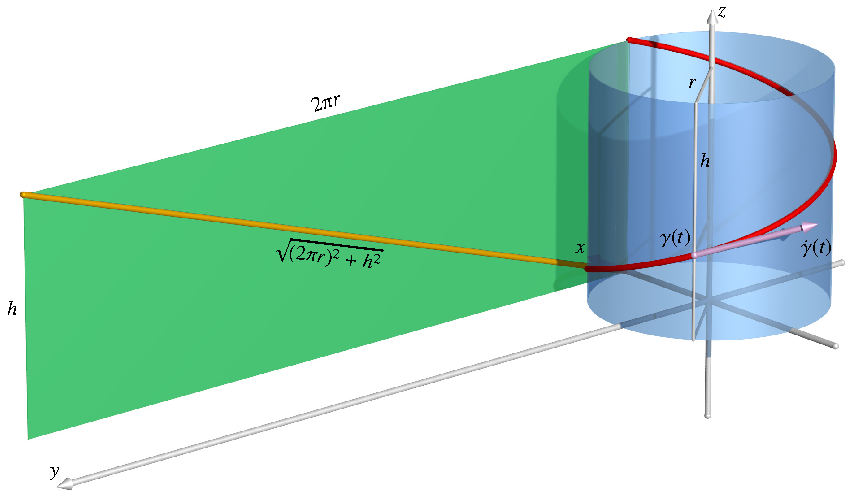
\includegraphics[width=\textwidth]{chapters/030-geometrie/images/zylinder.pdf}
\caption{Schraubenlinie mit der Parameterdarstellung
\eqref{buch:geometrie:eqn:helix} und Abrollung zur Berechnung der
Länge der Kurve.
\label{buch:geometrie:fig:zylinder}}
\end{figure}
Die Abbildung~\ref{buch:geometrie:fig:zylinder} zeigt 
\begin{equation}
\gamma
\colon
[0,2\pi] \to \mathbb{R}^3
:
t\mapsto\begin{pmatrix}r\cos t\\ r\sin t\\ th/2\pi\end{pmatrix}
\label{buch:geometrie:eqn:helix}
\end{equation}
beschreibt eine Schraubenlinie oder Helix.
\index{Schraubenlinie}%
\index{Helix}%
Die Abbildung ist ganz offensichtlich differenzierbar und hat die
Ableitung
\begin{equation}
\frac{d}{dt}\gamma(t)
=
\dot{\gamma}(t)
=
\begin{pmatrix} -r\sin t \\ r\cos t \\ h/2\pi\end{pmatrix}.
\label{buch:geometrie:eqn:helixdot}
\end{equation}
Die Länge dieser Schraubenlinie lässt sich direkt berechnen.
Die Schraubenlinie liegt auf dem Mantel eines Zylinders mit
Radius $r$ und Höhe $h$.
Durch Abrollen des Zylinders erkennt man, dass die Schraubenlinie
die Hypothenuse eines rechtwinkligen Dreiecks mit Katheten 
$2\pi r$ und $h$ ist.
Die Länge $l$ der Schraubenlinie ist daher
\begin{equation}
l = \sqrt{(2\pi r)^2 +h^2}
\label{buch:geometrie:eqn:helixlaenge}
\end{equation}
nach dem Satz von Pythagoras.
\end{beispiel}

Unterteilt man das Intervall $I$ in den Teilpunkten $t_i$ mit
\[
a = t_0 < t_1 < t_2 < \dots < t_{n-1} < t_n = b,
\]
dann ist die Summe
\[
L
=
\sum_{i=0}^{n-1} |\gamma(t_{i+1}) - \gamma(t_{i})|
\]
eine Approximation für die Länge der Kurve.
Die Differenz auffeinanderfolgender Punkte kann mit Hilfe der
Ableitung als
\[
\gamma(t_{i+1})-\gamma(t_i)
\approx
\dot{\gamma}(t_{i}) \cdot (t_{i+1}-t_i)
\]
approximiert werden.
Damit wird die Summe $L$ approximiert durch
\[
L\approx \sum_{i=0}^{n-1} |\dot{\gamma}(t_i)| \cdot (t_{i+1}-t_i).
\]
Dies ist eine Riemannsche Summe für das Integral
\[
\int_a^b |\dot{\gamma}(t)|\,dt,
\]
wir definieren die Bogenlänge einer Kurve daher wie folgt.

\begin{definition}
\label{buch:geometrie:def:kurvenlaenge}
Sei $\gamma\colon I\to\mathbb{R}$ eine Kurve im Sinne der
Definition~\ref{buch:geometrie:def:kurve}.
Dann ist die {\em Bogenlänge} entlang der Kurve zwischen dem Punkt
$\gamma(a)$ und $\gamma(t)$ definiert durch das
Integral
\[
l(t) = \int_{a}^t |\dot{\gamma}(\tau)|\,d\tau.
\]
\end{definition}

\begin{beispiel}
Die Helix mit der Parametrisierung~\eqref{buch:geometrie:eqn:helix}
hat die Kurvenlänge
\begin{align*}
l(t)
&=
\int_0^t |\dot{\gamma}(\tau)|\,d\tau
=
\int_0^t \sqrt{r^2\sin^2 \tau + r^2\cos^2\tau + (h/2\pi)^2}\,d\tau
\\
&=
\int_0^t \sqrt{r^2 + (h/2\pi)^2}\,d\tau
=
t\sqrt{r^2+(h/2\pi)^2}.
\end{align*}
Für eine ganze Umdrehung, also für $t=2\pi$ finden wir
\(
l(2\pi) = \sqrt{4\pi^2 r^2 + h^2},
\)
was mit dem elementaren Resultat~\eqref{buch:geometrie:eqn:helixlaenge}
übereinstimmt.
\end{beispiel}

\subsubsection{Länge eines Graphen}
Der Graph einer auf dem Intervall $I=[a,b]$ definierte Funktion
$y=f(x)$ kann als Parametrisierung einer Kurve
\[
\gamma
\colon
[a,b] \to \mathbb{R}^2
:
x \mapsto \begin{pmatrix}x\\f(x)\end{pmatrix}
\]
betrachtet werden.
Nach Definition~\ref{buch:geometrie:def:kurvenlaenge}
ist Länge dieser Kurven zwischen den Punkten $(a,f(a))$ und $(x,f(x))$
durch das Integral
\[
l(x)
=
\int_a^x \biggl| \begin{pmatrix}1\\f'(\xi)\end{pmatrix}\biggr|\,d\xi
=
\int_a^x \sqrt{1+f'(\xi)^2}\,d\xi
\]
gegeben.

\begin{beispiel}
Die auf dem Intervall $I=[0,b]$ definierte quadratische Funktion $f(x)=cx^2$
mit $b>0$ und $c>0$ hat die Bogenlänge
\begin{align*}
l(x)
&=
\int_0^x \sqrt{1+f'(\xi)^2}\,d\xi
=
\int_0^x \sqrt{1+4c^2\xi^2}\,d\xi
=
\biggl[
\frac{ \operatorname{arsinh}2c\xi)}{4c} + \frac{\xi\sqrt{4c^2\xi^2+1}}{2}
\biggr]_0^x
\\
&=
\frac{ \operatorname{arsinh}(2cx)}{4c}.
\end{align*}
Die Stammfunktion wurde mit einem Computeralgebraprogramm gefunden.
\end{beispiel}

\subsubsection{Kurvenlänge in Polarkoordinaten}
Eine Kurve kann in Polarkoordinaten in der Ebene durch eine Funktion
$r=r(\varphi)$ beschrieben werden.
Dies führt auf eine Parametrisierung
\[
\varphi \mapsto \gamma(\varphi)=\begin{pmatrix}
r(\varphi)\cos\varphi\\
r(\varphi)\sin\varphi
\end{pmatrix}
\]
durch den Polarwinkel $\varphi$.
Die Kurvenlänge kann gemäss 
Definition~\label{buch:geometrie:def:kurvenlaenge} braucht
die Ableitung der Parametrisierung, also die Funktion
\[
\dot{\gamma}(\varphi)
=
\begin{pmatrix}
r'(\varphi)\cos\varphi - r(\varphi)\sin\varphi\\
r'(\varphi)\sin\varphi + r(\varphi)\cos\varphi
\end{pmatrix}.
\]
Die Länge von $\dot{\gamma}$ ist
\begin{align*}
|\dot{\gamma}(\varphi)|^2
&=
\bigl(
r'(\varphi)\cos\varphi - r(\varphi)\sin\varphi
\bigr)^2
+
\bigl(
r'(\varphi)\sin\varphi + r(\varphi)\cos\varphi
\bigr)^2
\\
&=
r'(\varphi)^2\cos^2\varphi
-2r(\varphi)r'(\varphi)\cos\varphi\sin\varphi
+r(\varphi)^2\sin^2\varphi
\\
&\qquad
+r'(\varphi)^2\sin^2\varphi
+2r(\varphi)r'(\varphi)\sin\varphi\cos\varphi
+r(\varphi)^2\cos^2\varphi
\\
&=r'(\varphi)^2(\cos^2\varphi+\sin^2\varphi)
+ r(\varphi)^2(\sin^2\varphi+\cos^2\varphi).
\\
&=
r'(\varphi)^2 + r(\varphi)^2.
\end{align*}
Dies führt auf das
Integral
\begin{equation}
l(\alpha)
=
\int_a^\alpha \sqrt{r'(\varphi)^2 + r(\varphi)^2}\,d\varphi
\end{equation}
für die Länge der Kurve.

\subsection{Kreis}
Die Länge eines Bogens auf dem Einheitskreis zwischen dem Punkt
$(1,0)$ und $P=(x,y)$ mit $x^2+y^2=1$ ist nach Definition der
Winkel $\alpha$ zwischen der $x$-Achse und $P$.
Es gilt also
\[
\tan\alpha = \frac{y}{x}
\qquad\text{oder}\qquad
\sin\alpha = y = \sqrt{1-x^2}.
\]
Der Kreis kann auch als Graph $y=f(x)=\sqrt{1-x^2}$ parametrisiert werden,
in der die Länge des Bogens 
\begin{align*}
l(x)
=
\int_x^1 \sqrt{1+f'(t)^2}\,dt
=
\int_x^1 \sqrt{1+\frac{t^2}{1-t^2}}\,dt
=
\int_x^1 \sqrt{\frac{1-t^2+t^2}{1-t^2}}\,dt
=
\int_x^1 \frac{dt}{\sqrt{1-t^2}}.
\end{align*}
Aus dem bekannten Wert der Länge des Bogens erhalten wir jetzt die
Formel
\begin{equation}
\arcsin \sqrt{1-x^2} = \int_x^1 \frac{dt}{\sqrt{1-t^2}}.
\label{buch:geometrie:eqn:kreislaenge} 
\end{equation}
Tatsächlich ist die Ableitung davon
\[
\frac{d}{dx}\arcsin\sqrt{1-x^2}
=
-\frac{1}{\sqrt{1-x^2}},
\]
was mit der Integralformel~\ref{buch:geometrie:eqn:kreislaenge} 
übereinstimmt.

\subsection{Hyperbeln und Ellipsen
\label{buch:geometrie:subsection:hyperbeln-und-ellipsen}}
Die Funktion $f(x)=\sqrt{1+x^2}$ beschreibt eine gleichseitige
Hyperbel.
Die Bogenlänge zwischen dem Punkt $(0,1)$ und $(x,y)$ auf der
Hyperbel ist gegeben durch das Integral:
\[
l(x)
=
\int_0^x \sqrt{1+f'(t)^2}\,dt
=
\int_0^x \sqrt{1+\frac{t^2}{1+t^2}}\,dt
=
\int_0^x \sqrt{\frac{1+2t^2}{1+t^2}}\,dt.
\]
Dieses Integral ist nicht in geschlossener Form lösbar.
Natürlich können auch andere Parametrisierungen für die Hyperbel
verwendet werden, die entstehenden Integrals, dies ändert jedoch
nichts an der Schwierigkeit, einen Ausdruck für den Wert des
Integrals anzugeben.

Für eine Ellipse kann man die Parameterdarstellung 
\[
t\mapsto \begin{pmatrix}a\cos t\\b\sin t\end{pmatrix}
\]
verwenden.
Die Länge eines Ellipsenbogens zwischen den Winkelargumenten $\alpha$ und
$\beta$ ist dann
\[
l(\alpha,\beta)
=
\int_\alpha^\beta
\sqrt{
a^2 \sin^2 t + b^2 \cos^2t
}
\,dt
=
a
\int_\alpha^\beta
\sqrt{
\sin^2 t + \frac{b^2}{a^2} \cos^2t
}
\,dt.
\]
Auch dieses Integral ist nicht in geschlossener Form lösbar.
Dies motiviert in Kapitel~\ref{buch:chapter:elliptischefunktionen}
die Definition~\ref{buch:elliptisch:def:integrale123}
der sogenannten elliptischen Intefrale als neue
spezielle Funktionen.
Auf Seite~\pageref{buch:elliptisch:fig:ellipsenumfang} wird gezeigt,
dass der Umfang einer Ellipse $aE(b/a)$ ist (siehe auch
Abbildung~\ref{buch:elliptisch:fig:ellipsenumfang}).





%
% flaeche.tex
%
% (c) 2021 Prof Dr Andreas Müller, OST Ostschweizer Fachhochschule
%
\section{Flächeninhalt
\label{buch:geometrie:section:flaeche}}
\rhead{Flächeninhalt}
Die elementare Definition des Integrals versucht, den Flächeninhalt
unter dem Graphen der Funktion $y=f(x)$ zu definieren.
Die Erfahrung zeigt, dass es nicht immer einfach ist, ein Integral in
geschlossener Form zu berechnen.
Solche Integrale können auf sinnvolle neue spezielle Funktionen führen.

\subsection{Berechnung des Flächeninhaltes in kartesischen Koordinaten}
Wir betrachten in diesem Abschnitt nur die Berechnung des
Flächeninhaltes von Teilgebieten der Ebene $\mathbb{R}^2$
aus ihrer Berandung.
Sei $\gamma\colon I \to\mathbb{R}^2$ eine Kurve und 
\[
a=t_0<t_1<t_2<\dots t_{n-2}<t_{n-1}<t_n=b
\]
eine Unterteilung des Intervalls.
Die Kurve muss ausserdem geschlossen sein, also $\gamma(a)=\gamma(b)$.
Die Punkte $\gamma(t_i)$ sind die Ecken eines Polygons, das die gesucht
Fläche approximiert.

Der Flächeninhalt des Polygons kann mit der Schuhbändelformel
\cite[p.~184]{buch:linalg}
berechnet werden.

\begin{align*}
F
&=
\sum_{i=0}^{n-1}
\frac12
\biggl|\begin{matrix}
x(t_i)    &y(t_i)    \\
x(t_{i+1})&y(t_{i+1})
\end{matrix}\biggr|
\approx
\frac12
\sum_{i=0}^{n-1}
\biggl|\begin{matrix}
x(t_i)    &y(t_i)    \\
x(t_{i+1})-x(t_i)&y(t_{i+1})-y(t_i)
\end{matrix}\biggr|
\\
&=
\frac12
\sum_{i=0}^{n-1}
\biggl|\begin{matrix}
x(t_i)                        &y(t_i)    \\
\dot{x}(t_{i+1}) (t_{i+1}-t_i)& \dot{y}(t_{i+1}) (t_{i+1}-t_i)
\end{matrix}\biggr|
\\
&=
\frac12
\sum_{i=0}^{n-1}
\biggl|\begin{matrix}
x(t_i)           &y(t_i)    \\
\dot{x}(t_{i+1}) & \dot{y}(t_{i+1})
\end{matrix}\biggr|
(t_{i+1}-t_{i})
\end{align*}
Die letzte Summe kann als Riemann-Summe und damit als Approximation für
das Integral
\[
F
\approx
\frac12
\int_a^b
\left|\begin{pmatrix} x(t)&y(t)\\\dot{x}(t)&\dot{y}(t)\end{pmatrix}\right|
\,dt
\]
gesehen werden.
Der Flächeninhalt des Gebietes, welches von der Kurve $\gamma$
berandet wird, ist daher
\begin{equation}
F
=
\frac12
\int_a^b x(t)\dot{y}(t)-y(t)\dot{x}(t)\,dt.
\label{buch:geometrie:eqn:flaeche}
\end{equation}

Die Formel~\eqref{buch:geometrie:eqn:flaeche} gilt auch für nicht
geschlossene Kurven.
Sie berechnet dann den Flächeninhalt eines Gebietes, welches von
der Strecke vom Ursprung zu $\gamma(a)$, der Kurve von $\gamma(a)$ nach
$\gamma(b)$ und von der Strecke von $\gamma(b)$ zurück zum Nullpunkt
berandet wird.

\begin{beispiel}
Der Flächeninhalt eines Kreissektors mit Öffnungswinkel $\alpha$ ist
kann mit Hilfe der Parametrisierung
\[
\gamma
\colon
[0,\alpha] \to \mathbb{R}^2
:
t\mapsto \begin{pmatrix}r\cos t\\ r\sin t\end{pmatrix}
\]
berechnet werden.
Das Integral~\eqref{buch:geometrie:eqn:flaeche} wird dann zu
\begin{align*}
F
&=
\frac12
\int_0^\alpha r\cos t \cdot r\cos t - r\sin t \cdot (-r\sin t)\,dt
\\
&=
\frac{r^2}2
\int_0^\alpha
\cos^2t + \sin^2t\,dt
=
\frac{r^2\alpha}2,
\end{align*}
wie erwartet.
\end{beispiel}

\subsubsection{Flächeninhalt in Polarkoordinaten}
Ist die Kurve in Polarkoordinaten durch die Funktion
$\varphi\mapsto r(\varphi)$ gegeben, dann kann man $\varphi$ als
Parameter verwenden.
Die Determinante in der Flächenformel wird
\begin{align*}
\biggl|
\begin{matrix}
x(t_i)& y(t_i)\\
\dot{x}(t_i)& \dot{y}(t_i)
\end{matrix}
\biggr|
&=
\biggl|
\begin{matrix}
r(\varphi)\cos\varphi&r(\varphi)\sin\varphi\\
-r(\varphi)\sin\varphi+r'(\varphi)\cos\varphi
	&r(\varphi)\cos\varphi+r'(\varphi)\sin\varphi
\end{matrix}
\biggr|.
\end{align*}
Der Integrand in der Flächenformel wird dann
\[
\frac12\bigl(
r(\varphi)^2 \cos^2\varphi +r(\varphi)r'(\varphi)\cos\varphi\sin\varphi
+
r(\varphi)^2 \sin^2\varphi -r(\varphi)r'(\varphi)\sin\varphi\cos\varphi
\bigr)
=
\frac{r(\varphi)^2}2
\]
und die Fläche kann mit
\[
F(\alpha,\beta)=\int_\alpha^\beta \frac{r(\varphi)^2}{2}\,d\varphi
\]
berechnet werden.

\subsection{Flächeninhalt von Ellipsen und Hyperbeln}
Ellipsen und Hyperbeln sind besonders einfach zu parametrisieren und
damit ist auch die Fläche, die von Ellipsen oder Hyperbeln berandet
wird, besonders einfach zu berechnen.

\subsubsection{Ellipse}
Für die Ellipse mit der Gleichung
\[
\frac{x^2}{a^2}+\frac{y^2}{b^2}=1
\]
kann man mit der Parametrisierung
\[
\gamma\colon
[0,2\pi] \to \mathbb{R}^2
:
t \mapsto \begin{pmatrix}a\cos t\\ b\sin t\end{pmatrix}
\]
beschreiben.
Einen Sektor zwischen den Winkeln $\alpha$ und $\beta$
\begin{align*}
F
&=
\int_\alpha^\beta a\cos t \cdot b\cos t-b\sin t\cdot (-a\sin t)\,dt
\\
&=
ab
\int_\alpha^\beta \cos^2 t + \sin^2 t\,dt
=ab(\beta-\alpha).
\end{align*}
Dieses Resultat ist auch rein geometrisch leicht nachzuvollziehen:
Der Sektor entsteht dadurch, dass man ein Kreissektor mit Radius $a$
entlang der $y$-Achse um den Faktor $b/a$ gestaucht wird.
Aus dem Flächeninhalt $a^2(\beta-\alpha)$ des Kreissektors wird dann
der Flächeninhalt $a^2(\beta-\alpha)\cdot \frac{b}{a}=ab(\beta-\alpha)$.

\subsubsection{Hyperbel}
\begin{figure}
\centering
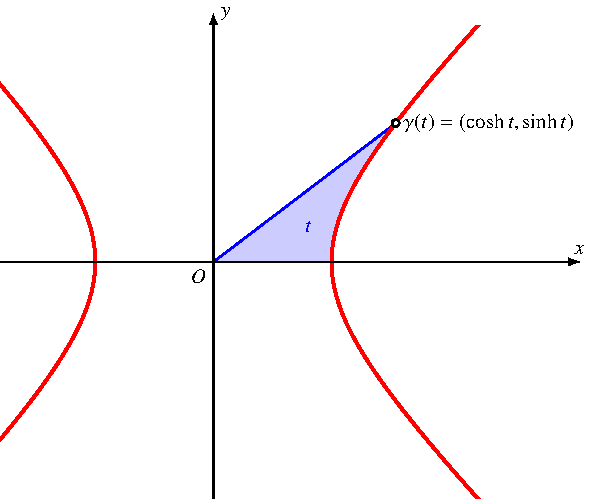
\includegraphics{chapters/030-geometrie/images/hyperbelflaeche.pdf}
\caption{Das Argument $t$ der hyperbolischen Funktionen ist der Inhalt
des krummlinig berandeten Dreiecks, bestehend aus der Strecke 
vom Nullpunkt $O$ zum Punkte $(1,0)$, dem Hyperbelbogen bis zum
Punkt $\gamma(t)=(\cosh t,\sinh t)$ und schliesslich der Strecke
von $\gamma(t)$ zurück zum Nullpunkt.
\label{buch:geometrie:fig:hyperbelflaeche}}
\end{figure}
Die hyperbolischen Funktionen geben eine einfache Parametrisierung
der in Abbildung~\ref{buch:geometrie:fig:hyperbelflaeche}
dargestellten Hyperbel mit der Gleichung
\(
x^2-y^2=1
\).
Der in der Abbildung blau hervorgehobene Flächeninhalt ist der Wert
des Integrals
\begin{align*}
F(t)
&=
\int_0^t
\biggl|
\begin{matrix}
\cosh s&\sinh s\\
\sinh s&\cosh s
\end{matrix}
\biggr|
\,ds
=
\int_0^t
\cosh^2s-\sinh^2s\,ds
=
\int_0^t ds = t.
\end{align*}
Das Argument $t$ der hyperbolischen Funktionen ist also der Flächeninhalt
des von der Hyperbel krummlinig berandeten Dreiecks.
Daher heissen die Umkehrfunktionen der hyperbolischen Funktionen
$\operatorname{arsinh}y$ und $\operatorname{arcosh}y$, Abkürzung
für {\em area cuius sinus hyperbolicus $y$ est}, Fläche, deren zugehöriger
Wert des Sinus hyperbolicus $y$ ist.

\subsubsection{Fokalgleichung in Polarkoordinaten}
\begin{figure}
\centering
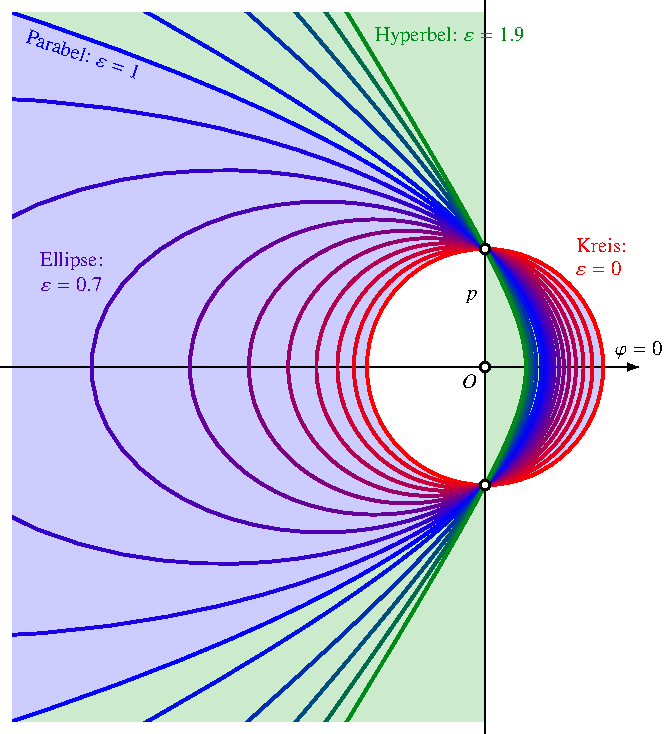
\includegraphics{chapters/030-geometrie/images/polargleichung.pdf}
\caption{Polargleichung der Kegelschnitte mit konstantem Wert für den
Parameter $p$ und verschiedene Werte der Exzentrizität $\varepsilon$.
Der Kreis (rot) hat Exzentrizität $\varepsilon=0$,
die Parabel (blau) hat $\varepsilon=1$.
Für $0<\varepsilon<1$ entstehen Ellipsen, die im blauen Bereich liegen,
für $\varepsilon>1$ entstehen Hyperbeln, die im grün hinterlegten Teil
der Ebene liegen.
\label{buch:geometrie:fig:polargleichung}}
\end{figure}
Das zweite Keplersche Gesetz über Planetenbahnen besagt, dass sich ein
Planet auf seiner elliptischen Bahn um die Sonne so bewegt, dass
sein Radiusvektor in gleichen Zeiten gleiche Flächen überstreicht.
Die bisher verwendete Parametrisierung hat den Mittelpunkt der Ellipse
im Nullpunkt, nach dem ersten Keplerschen Gesetz ist aber müssen
wir eine Parametrisierung verwenden so, dass der Brennpunkt im
Ursprung liegt.
In Polarkoordinaten ist
\begin{equation}
r(\varphi) = \frac{p}{1+\varepsilon \cos\varphi}
\label{buch:geometrie:eqn:polargleichung}
\end{equation}
die sogenannte {\em Polargleichung} für die Kegelschnitte.
Für $\varepsilon=0$ wird $r(\varphi)=p$ konstant, die Gleichung
beschreibt in diesem Fall einen Kreis.
Für $\varepsilon=1$ entsteht eine Parabel.
Werte zwischen $0$ und $1$ parametrisieren Ellipsen mit verschiedener
Exzentrizität, Werte grösser als $1$ führen auf Hyperbeln.
Abbildung~\ref{buch:geometrie:fig:polargleichung} zeigt alle vier Fälle.

Die zwischen den Polarwinkeln $\alpha$ und $\beta$ überstrichene Fläche
wird durch das Integral
\[
F(\alpha,\beta)
=
\int_\alpha^\beta
\frac{r(\varphi)^2}2
\,d\varphi
=
\frac12 \int_\alpha^\beta
\frac{p^2 \,d\varphi}{(1+\varepsilon\cos\varphi)^2}
\]
Das Integral kann in geschlossener Form angegeben werden, die Formeln
sind aber ziemlich kompliziert und für uns hier nicht weiter nützlich.





\section*{Übungsaufgaben}
\rhead{Übungsaufgaben}
\aufgabetoplevel{chapters/030-geometrie/uebungsaufgaben}
\begin{uebungsaufgaben}
%\uebungsaufgabe{0}
\uebungsaufgabe{1}
\uebungsaufgabe{2}
\uebungsaufgabe{3}
\end{uebungsaufgaben}

